\chapter{Keeping Cool}
When I was growing up, in the 1950s, summers were extremely hot in
Panipat. At that time, Panipat was a Tehsil in district Karnal, Punjab,
and is now a district by itself in Haryana, India. 

The deep chill in December and January made us all pray for warmer
weather. Be careful what you ask for! It starts warming up in February; by
May and June, the temperature rises to 100 degrees F or more and stay
there, with bright sun glaring down every day. 

Even though almost seven decades have passed, it seems like it happened
only yesterday and I can visualize, feel and immersed in that time. 
 
We have a variety of ways to stay cool. Mercifully, none of us knows the
words like air conditioner or air cooler. As a result, there is no problem
of comparison with others. 

In the 1950s nobody is complaining much about the hot loo (burning hot
air) that hits our faces when we step out of the shade of the house. No
one knows or cares to know what the temperature is in Celsius or
Fahrenheit. We simply say “Bhai, is saal tthaan kamal di garmi payee aye"
(Brother, this year the heat is unusual). And we say the same thing every
year. It is just burning hot, and everyone talks impatiently about the
upcoming rain, which cools down the place. Cartoons showing eggs being
cooked on the roads are printed in newspaper. 
 
Everyone is saying "Is saal barshan late ho gayiyaan nein" (The rains are
late this year). And we say that every year. Everyday we look to the west
looking for a floating cloud that may be an early soldier announcing big
army of clouds and the onset of Monsoon. Our prayers are finally answered
and we see a wave of black clouds at the horizon, thunderously making
their way towards us. Finally the lightning and thunder are signals for my
siblings and I to run in, shed our clothes to bare minimum for decent
public exposure, and then run out. Some younger boys come out screaming
and jumping, totally naked. There is excitement in the air. Even radio is
playing happy songs of monsoon. 
 
Initially, the big splattering drops raise small plumes of dust from the
parched ground into the air, making it emit an unforgettable,
indescribable smell of the first rain. It is as if the thirsty dry earth
is saying "Thank you.” The single drops, a promise of outpouring of water
from the dark sky, sometimes leads to nothing more than that. To the
disappointment of all, the clouds change direction, go elsewhere, and make
someone else happy. We feel sad, but know that more are around the corner,
and our turn will come soon. 

When they finally come , no one cares or even knows about the fatal effect
of lightning strikes. We are out in droves in the open spaces and streets
and soak the sheets of water falling from the dark sky.
 
Soon the the open naaliyaan (open sewer lines) are overflowing. Small
brown rivulets have formed giving birth to large puddles and ponds. 

Swirls of black clouds, accompanied by an orchestra of thunders preceded
by lightning flashes, which look like dancing branches playing hide and
seek, let loose the much appreciated water. 

All the children and some adults, for hours, run around in the water. Even
cows and buffaloes take dips in the ponds to cool off. To our amazement,
dogs are swimming in the pond. They come out, shake their heads, spraying
water around them. But then they jump right back as more have joined the
group. 
 
We had already stocked up on paper boats, later made famous in a Jagjit
Singh’s song, well in advance of the first rain drop. They are now ready
to float. We let them loose, and run after them amidst sounds of thunder
and laughter. We catch them, empty out the pouring water from the boats,
and let them float a bit longer. But then the undulating waves and rain
drops overpower them. 

We waddle out, dripping water into the house, pick up the remainder of the
boats and start the fun all over. Squeals of joy fill the air. 
 
PitaJi, my father, is ready with bucketfuls of washed choosa (sucking
type) mangoes. Getting soaked in the rain or standing under open roof
spout, parnala, in the central part of the house, we roll the mangoes
between the palms to loosen the pulp, bite and spit a small piece on the
top, and suck out the pulp. We don’t need knives. The ones with faster
hands and mouths gets to eat more. The four brothers and their happy
father devour them, throwing the pits and skin in the flowing water. 

One such pit later took roots and became a source of future supplies. 

The mangoes vanish quickly, prompting PitaJi to run in and bring more from
the house, till none was left. 
 
\begin{figure}
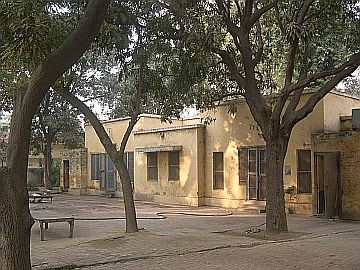
\includegraphics[width=.75\textwidth]{keeping_cool_pic_1.jpg}
\caption{Luthra home in Panipat, 1950s} \end{figure}


Eventually, MataJi, my mother, calls all our names as a one liner – "Vey
VirinderKrishanGindiShoki hun andar aa jao, garam garam Poorhe te kheer
tayyar aye" (Hey Virinder, Krishan, Gindi, Shoki – come in now. Hot poorhe
and rice pudding are ready.”)
 
We all run in, make the floor soaking wet, take a quick shower with the
water carefully saved in the large oval galvanized iron tub and several
metal buckets. 

Water from the taps comes for one hour in the morning and one in the
afternoon. We leave the tap in the open position. At the first
intermittent hissing sound of air coming out ahead of the precious
commodity flowing through, we run to the three tootiyaan (faucets) in the
house. We fill every container of every size and shape with water. 

We schedule bathing in the tap water around the times when it bubbles out
of the faucets. 

Large water storage tanks on the roof tops and motor pumps to transport
the water up came much later. 
 
We save water in the containers for later use, such as the one now
required, before the kheer and poorha, which we enjoy in the open veranda,
watching the rain gradually stop. It is amazing how all the puddles and
ponds get soaked up quickly by the thirsty land, plants, and trees. 
 
On lucky days we get hot jalebis purchased from local sweet maker, Bosa
Ram. We never have to pay him any cash. Unknown to us, he kept a running
account book in a long red cloth covered ledger, for us as well as all the
people living in our mohalla (neighbourhood). At the end of the month,
PitaJi paid the bills. We grew up thinking that Bosa Ram was such
a generous man giving away free sweets. 

He actually is a sweet man, always smiling and handing out a freebee or
two to us, especially boondi ke laddoo on Tuesdays, the day of god
Hanuman.
 
The first rain is a matter of rejoicing. The school principals declares
this day as a Fine Day. He declares the school closed. “Children, it is
a fine day. You can go home, enjoy the rain and have a fine day.” These
are melodious words to the children. We all hurriedly pack up our bustas
(school bags), and run home. There are no school buses, no pick ups, no
telephones to alert the parents. It is completely safe for everyone. All
the children, noisily, run or walk home. 

On later rainy days, children plead “Principal sahib, it is a Fine Day,
may we go home.” Depending on his mood, children run out with glee or sulk
and stayed in school. 
 
The abundant water transported by the clouds brings joy to all living
objects. Life is a double faced coin, pleasure and pain run side by side.
Occasionally we hear about someone drowning, some areas get flooded by
overflowing rivers and creeks. There are no dams to regulate the ocean
being unloaded on the land. 

We never faced such life changing calamities, but had our share of minor
annoyances. The solid appearing concrete roof of our house is obviously
not water tight. Water drips through into all the rooms from the lowest
parts of the uneven ceiling. We hurriedly move around our precious
furniture of 10 wooden chairs, a table and two beds. What cannot be moved,
gets covered by plastic sheets. We strategically place all available
containers, large and small, to catch the drips. Everyone is running in
and out, emptying the rapidly filling containers. Finally the clouds
declare the end of their show. 

Panipat is located on flat land and there is nothing to obstruct the
display of nature's panoramic display of receding clouds, a hazy sunshine
and colourful display of all its colours in the semi-circular rainbow from
one part of horizon to the other. Some days we are gifted two rainbows in
all their glory. 
 
The cool air stays for a while. Then the heat, along with the newly added
humidity, returns with vengeance. Constant dripping sweat keeps our cotton
shirts and knickers (shorts) wet. We replenish it by drinking cool water
dispensed from the wide open clay round container – gharha or matka, and
from narrow long necked clay container – surahi. We have a wooden stand
that holds three of these containers. Their openings are carefully covered
with a steel plate, inverted katori, or cloth to protect the drinking
water from dust and thirsty flies. Being made of porous clay, they are
natural water coolers. 
 
A daily dose of Shikanjvi (lemon drink) is a must. We are lucky to use
freshly picked lemons from our own garden to make the sweet lemon drink
with the cool water. The young hands struggle to press the flat handled of
a wooden lemon squeezers. We are thrifty. The squeezed lemon pieces are
again stacked in the squeezer to get the last drop out. We are generous
with sugar to dilute the tangy taste of lemons; some people add a pinch of
salt as well. 
 
In the verandas and windows, we have Khas Khas chick, sometimes called
Tatti. We always laugh and wonder why such an aromatic mat is given such
a paradoxical name. This is made of a breed of grass that grows downwards,
and can attain a length between 6 to 8 feet. We fill buckets of water,
which we pour on the top of the chicks, letting it trickle down. The one
in the veranda has a cloth border with a rope attached at one end. We take
turns to sway it back and forth, letting air filter through it and bring
the cool fragrant air inside. The ones in the windows depend on the flow
of breeze. These are our natural fragrant air coolers.
 
We keep ceiling fans switches in the on position all the time. But it
doesn’t not mean that the fans swirl all the time, as it is common to hear
“Lao, bijli fir chali gayee aye" (There, electricity has gone again.)
Electricity runs through the wires intermittently with random
interruptions. “It is gone more than it comes” is a common complaint. 
 
As a backup, we have several ornate, rectangular or rounded, hand held
fans made of woven cane strips attached to sturdy polished wood handles.
Each one has different pattern of cloth border. Cheaper varieties without
cloth border and flayed borders are also available. Children happily sway
them back and forth for themselves and also help the elders as the
swirling motion of their fingers or wrist can easily tire the old hands.
In addition to providing movement to the air, these fans keep flies at
bay. 
 
We never stop playing outside, despite the heat or even the hanerian (dark
dust storms) that make their appearances in the weeks leading up to the
rainy season. There are many trees on our street, providing us the much
needed shade to play Bante (marbles). Other games such as Piththu, Guli
danda, and Cricket are saved till the air cools down a little, as the
orange sun moves towards the horizon. Three months of summer vacations
from school is heavenly respite from heat in the school and also provide
us plenty of time to play. 
 
We wear one of the two cotton white shirts and knickers we all have or
share. We wear one and MataJi, with regular help from a lady, Ganga Devi,
washes and dries the other. 

Mata Ji is always busy, from before sunrise to way past sunset, mostly
washing clothes and cooking. 
 
We take short baths two or three times a day to wash off the dust and also
to cool down the body. In the absence of constant running city water, we
draw water from the two hand pumps in case all the containers are empty. 
 
Street vendors are busy selling baraf de gole, (shaved crushed ice balls),
covered with multi-colour sugary syrups. Depending on how much money is
left over after buying the essentials, we sometimes indulge in this
luxury. 
 
The vendors also sell frozen kulfi pulled by the end of immersed wooden
stick out of conical metal containers, which are stored in ice filled
drums. It comes in plain variety or one mixed with pista (pistachio).
Spaghetti shaped Falooda is placed over the kulfi. It makes a delicious
cold combination. 
 
Some street vendors sell carbonated soda drinks, dispensed in ice chilled
glass bottles. These are way too expensive for our family. I might have
tasted the sweet soda water only once. The gas in the bottle is held in
check by a marble size glass ball in the narrow neck of the bottle. The
ball is pushed down using the thumb with force. Once, a bottle burst under
high pressure, and a friend of mine lost his one eye due to the injury
from broken glass. There are no eye surgeons in Panipat. 
 
Making ice cream at home is a highlight of the summer. Amongst many other
luxuries of life which our elder brother, Prem, brought home, everybody
loves the ice cream maker. It is a wooden drum with a metal container
inside. The revolving blades inside the metal container are attached to
a handle through a couple of gears.
 
Making ice cream is a big production. MataJi boils milk, mixed with cream;
later sugar and Kesar is added. Sometimes we have the luxury of adding cut
pieces of almonds or pistachios. When the mixture has cooled, we pour it
into the container. 

In the meantime, one of us pedals our bicycle to the ice cream factory
located about 2 miles from home. It seems much farther than that to small
legs and feet. We purchase a slab of ice, wrap it carefully in a sheet cut
out from a jute bag, and tie it securely to the carrier of the bicycle.
The return journey is brisk, lest all the ice should melt. Slow drips of
water are incentive to pedal harder. 
 
The team at home is eagerly waiting and ready with a metal hammer to
quickly crush the wrapped ice into small pieces. These pieces, along with
sprinkling of large salt granules, are placed between the metal container
and the outer wooden wall. 

Impatiently, we start rotating the handle, adding salt and ice, as it
melts and oozes out through the slits in the outer wooden container.
Initial rotations are peace of cake and easy and are assigned to the
younger children. The more muscular older children complete the job as the
churning blades become hard to move through freezing ice cream. 
 
Anticipation grows as the rotations becomes harder. When rotating becomes
almost impossible, this is a sign of joy and screams. Now, we all have
watering mouths. The lid of the container is opened, and a water laced
spoon, later replaced by a round one with a release handle, takes out the
ice cream. All of us have katoris and spoons ready on out stretched hands.
“Thodhi hore de de na.” (give me little bit more) we all request. We
relish it, eat it quickly to get a second helping and also before the heat
melts it down to milk. Almost always, we argue about who will scrape the
bottom portion of the container. We turn the container upside down to let
the last few drops trickle down into our thirsty mouths. Vanilla is our
favourite flavor. The taste and memory lingers. 
 
Sardai is another drink for the summer. We make it mostly when PitaJi
comes home for a couple of days from his job at the out of town brick
kilns. Water soaked, peeled almonds, cantaloupe seeds and black pepper are
crushed using Dauri Sota (mortar and pestle). Dauri is made of stone, and
Sota is a round smooth log of wood, 3 to 4 inch diameter and about two and
a half feet long. We occasionally use the sota as a weapon during the
sibling fights. 

The crushed powder is put in a jug. Water is added to make a paste, and
then we ad more water, which converted it into a drink. This is filtered
through a thin muslin cloth. Sugar and cool water (ice-if available from
Bosa Ram), are added and this makes a wonderful drink in the hot days. 
 
Another way to stay hydrated is to eat fruits rich in water. A large
watermelon, weighing about 30 to 35 pounds, is kept in cool water all day.
In the evening, the whole family sits together and eats all of it in one
go. We have no refrigerators to store the left overs. We eat cucumbers,
considered Thandi Sabzi (vegetable that cools you), every day. We cut the
top and rub it against the bare surface of the remainder for several
minutes; white foam erupts from the main body of the cucumber, which is
wiped away. This is supposed to remove the bitterness out of the cucumber. 
 
The sun mercifully sets. Preparations are made for a comfortable sleep.
Tired bodies need to revitalize and face the next hot day. 

All of us sleep outside in the yard. All the children sprinkle water
(Taraai) on the dry parched ground as well as the brick lined large yard.
We carry buckets filled with water which we sprinkle by hand, half on the
ground and merrily half on one another. The water settles the dust and
cools the hot grounds. The family lays out several charpais, four legged
beds made out of jute or nivaar (crisscrossed wide cotton bands). Two
sheets and a pillow make our bed. 
 
Mosquitoes are waiting for the victims. In our defence, we put up
Machchardanis, (mosquito nets.) Two bamboo sticks are anchored in the
shape of an X at the two ends of the bed. We tie the mosquito net to the
bamboo sticks using the attached cotton strips in the four corners. The
edges are carefully tucked under the sheet. Even a small opening means
listening to the swirling sounds of mosquitoes, as if alerting us to get
ready for the bite. 
 
The night time temperature drops quickly. A glass of ice cold milk,
sometimes with jalebi or bread, is our night cap. “Don't forget to rinse
your mouth”, ever vigilant MataJi says, and we obey. We don’t brush our
teeth but rinse several times, a vigorous polishing teeth with index
finger, swishing and rinsing is a must. Laying in beds, side by side, we
talk of the day's events and make plans for the next. Exhausted bodies go
off to sleep, and wake up to the sound of roosters and feeling of heat
from the sun. 
 
It is going to be another nice, hot day in Panipat and we are ready for
it.  
